%%%%%%%%%%%%%%%%%%%%%%%%%%%%%%%%%%%%%%%%%
% University/School Laboratory Report
% LaTeX Template
% Version 3.1 (25/3/14)
%
% This template has been downloaded from:
% http://www.LaTeXTemplates.com
%
% Original author:
% Linux and Unix Users Group at Virginia Tech Wiki 
% (https://vtluug.org/wiki/Example_LaTeX_chem_lab_report)
%
% License:
% CC BY-NC-SA 3.0 (http://creativecommons.org/licenses/by-nc-sa/3.0/)
%
%%%%%%%%%%%%%%%%%%%%%%%%%%%%%%%%%%%%%%%%%

%----------------------------------------------------------------------------------------
%	PACKAGES AND DOCUMENT CONFIGURATIONS
%----------------------------------------------------------------------------------------

\documentclass{article}

\usepackage[version=3]{mhchem} % Package for chemical equation typesetting
\usepackage{siunitx} % Provides the \SI{}{} and \si{} command for typesetting SI units
\usepackage{graphicx} % Required for the inclusion of images
\usepackage{natbib} % Required to change bibliography style to APA
\usepackage{amsmath} % Required for some math elements 
\usepackage[utf8]{inputenc}
\usepackage{tikz,pgfplots}
\usepackage[letterpaper, margin=0.5in]{geometry}
\usepackage{float}
\usepackage{enumitem}
\usepackage{gensymb}

% Roman numerials
\pagenumbering{arabic}

\setlength\parindent{0pt} % Removes all indentation from paragraphs

%\renewcommand{\labelenumi}{\alph{enumi}.} % Make numbering in the enumerate environment by letter rather than number (e.g. section 6)

%\usepackage{times} % Uncomment to use the Times New Roman font

% for some tables
\newcommand{\specialcell}[2][c]{%
  \begin{tabular}[#1]{@{}c@{}}#2\end{tabular}}
  
\providecommand{\e}[1]{\ensuremath{\times 10^{#1}}}
%----------------------------------------------------------------------------------------
%	DOCUMENT INFORMATION
%----------------------------------------------------------------------------------------

%\title{Determination of the Atomic \\ Weight of Magnesium \\ CHEM 101} % Title

%\author{John \textsc{Smith}} % Author name

%\date{\today} % Date for the report

\begin{document}

%\maketitle % Insert the title, author and date

% If you wish to include an abstract, uncomment the lines below
% \begin{abstract}
% Abstract text
% \end{abstract}

%----------------------------------------------------------------------------------------
%	SECTION 1
%----------------------------------------------------------------------------------------

\section{Objective}

To demonstrate the basic properties of strength and toughness by using the uniaxial tensile test and observing the necking and yielding behavior of the corresponding stress strain plots generated. To view and understand the micro structure of materials and the points of fraction using the Charpy Impact test and a scanning electron microscope. 

% If you have more than one objective, uncomment the below:
%\begin{description}
%\item[First Objective] \hfill \\
%Objective 1 text
%\item[Second Objective] \hfill \\
%Objective 2 text
%\end{description}

\section{Experimental Procedures}
\subsection{Rockwell hardness test}
LATER

\subsection{Charpy Impact test}
LATER

%----------------------------------------------------------------------------------------
%	SECTION 2
%----------------------------------------------------------------------------------------

\section{Experimental Results}
\begin{figure}[H]
\centering
\begin{tabular}{c || c | c | c | c | c | c | c}
Materials & \specialcell{$l_{0}$ \\ (in)} & \specialcell{$l_{f}$ \\ (in)} & \specialcell{$d_{0}$ \\ (in)} & \specialcell{$d_{f}$ \\ (in)} & \specialcell{strain rate \\ (in/s)} & \specialcell{Hardness \#1 \\ (RHN)} & \specialcell{Hardness \#2 \\ (RHN)} \\ \hline
Al-Cu & 1.908 & 2.275 & 0.254 & 0.232 & 0.005 & 14 & 19 \\ \hline
Steel-1018 & 1.884 & 2.477 & 0.233 & 0.206 & 0.005 & 31 & 31 \\ \hline
Steel-4340 & 1.973 & 2.008 & 0.235 & 0.234 & 0.001 & 72 & 74 \\ \hline
\end{tabular}
\caption{Uniaxial Tensile test results for all alloys}
\end{figure}

\begin{figure}[H]
\centering
\begin{tabular}{c || c}
& \specialcell{angle \\ ($\theta$)} \\ \hline
\specialcell{test run \\ (no sample)} & 159 \\ \hline
\specialcell{room \\ temperature} & 126 \\ \hline
\specialcell{liquid \\ nitrogen \\ temperature} & 156 \\ \hline
\end{tabular}
\caption{Charpy test results for Steel-1018}
\end{figure}

\begin{figure}[H]
\centering
\begin{tikzpicture}
\node at (0,0) {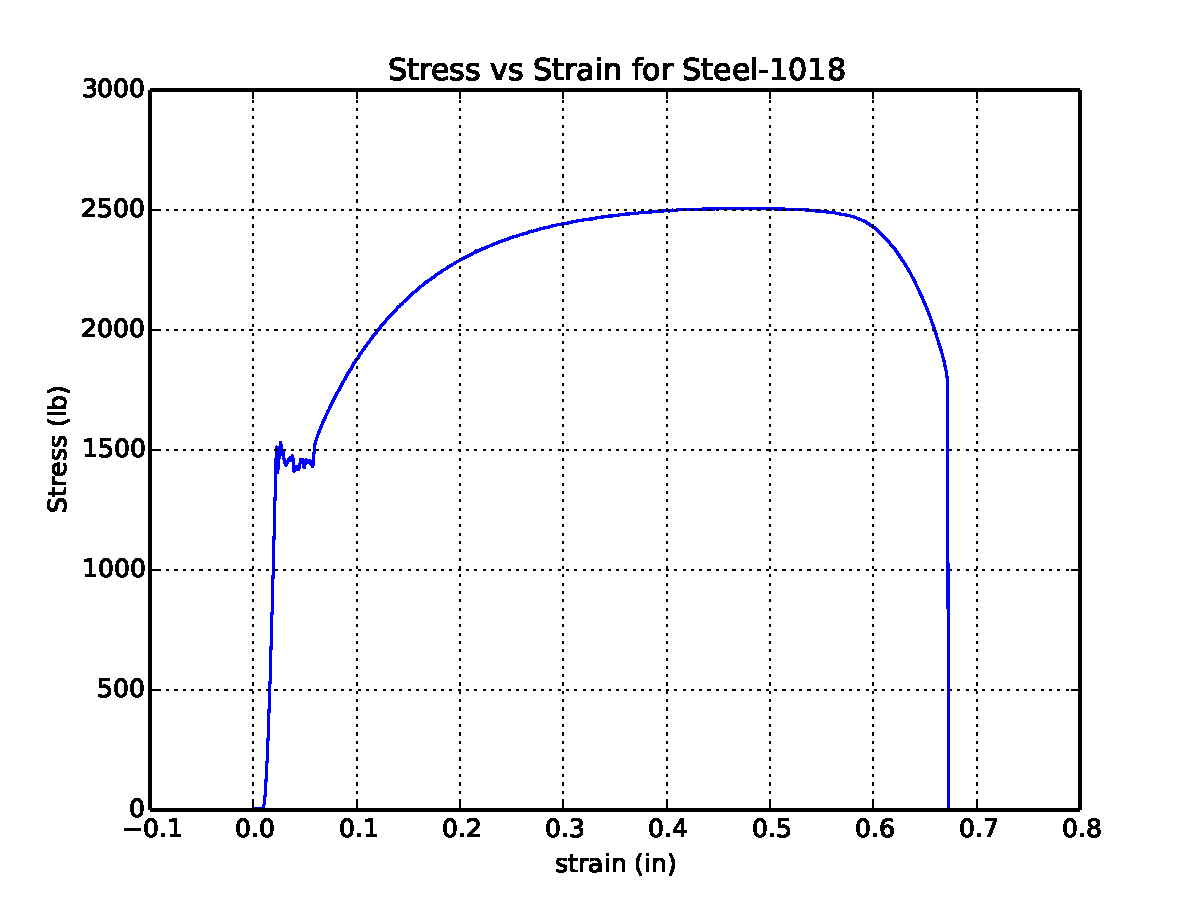
\includegraphics[width=225pt]{graphs/1018.pdf}};
\node at (8,0) {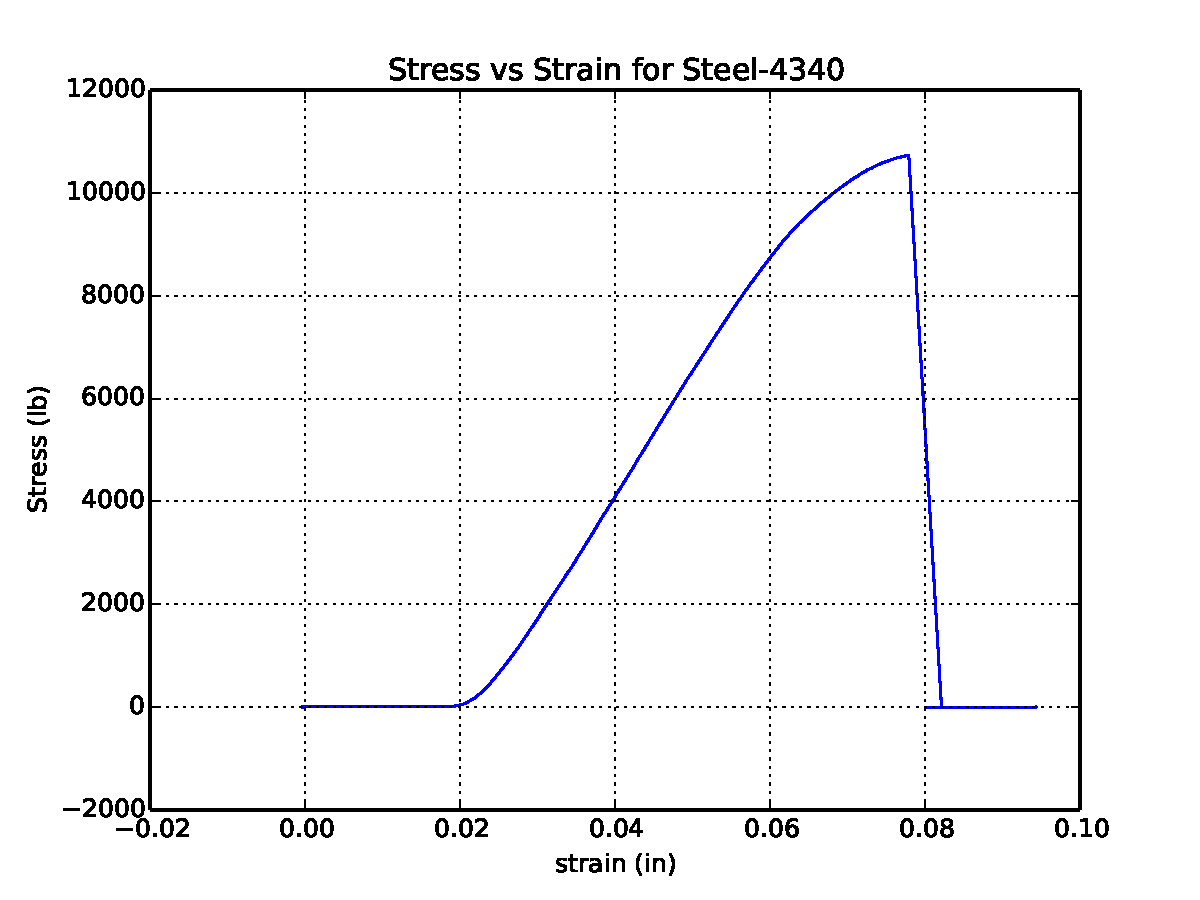
\includegraphics[width=225pt]{graphs/4340.pdf}};
\node at (4,-6) {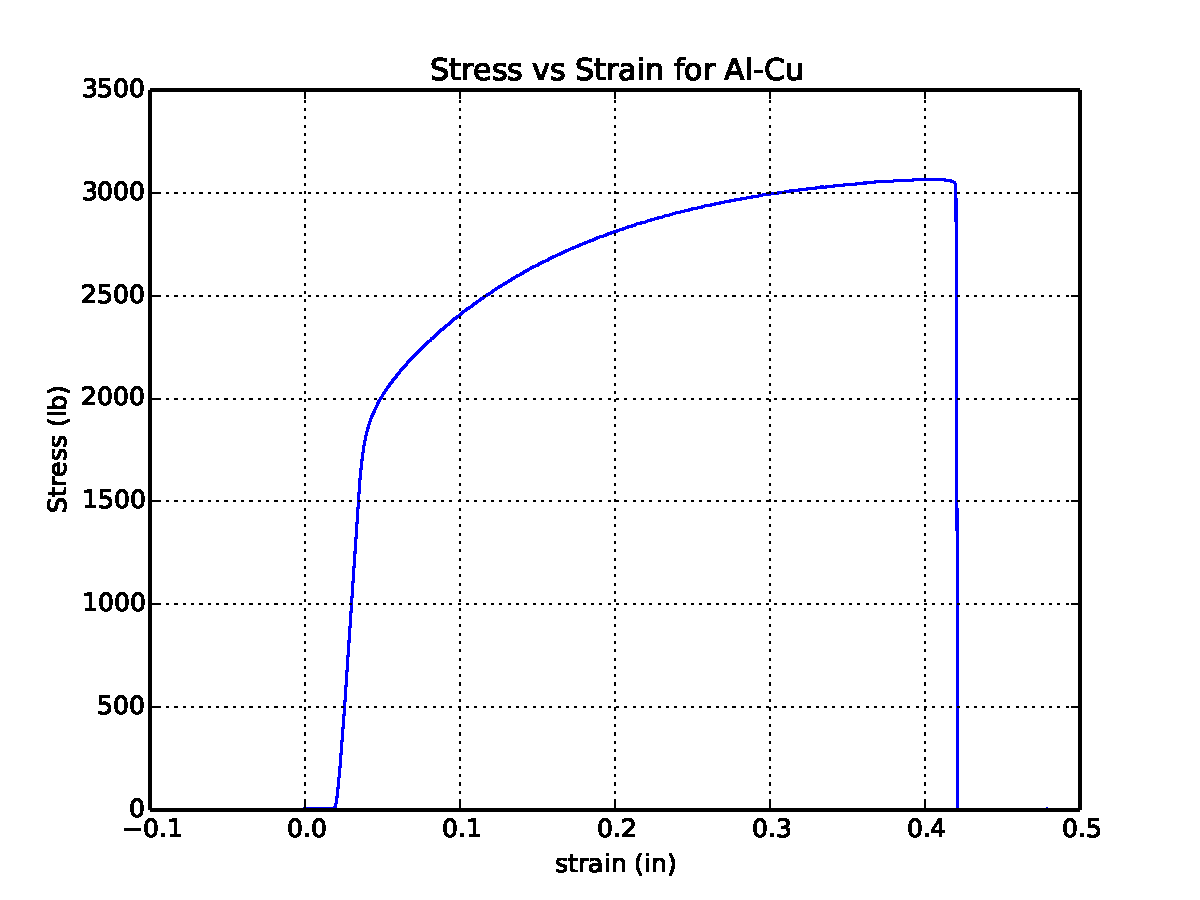
\includegraphics[width=225pt]{graphs/alcu.pdf}};
\node at (0,-3.3) {\textbf{(a)}};
\node at (8,-3.3) {\textbf{(b)}};
\node at (4,-9.3) {\textbf{(b)}};
\end{tikzpicture}
\caption{\textbf{(a)} Stress-Strain plot results for Steel-1018 using the uniaxial tensile test. \textbf{(b)} Stress-Strain plot for results for Steel-4340 using the uniaxial tensile test. \textbf{(c)} Stress-Strain plot results for Al-Cu alloy using the uniaxial tensile test.}
\end{figure}

\begin{figure}[H]
\centering
\begin{tikzpicture}
\node at (0,0) {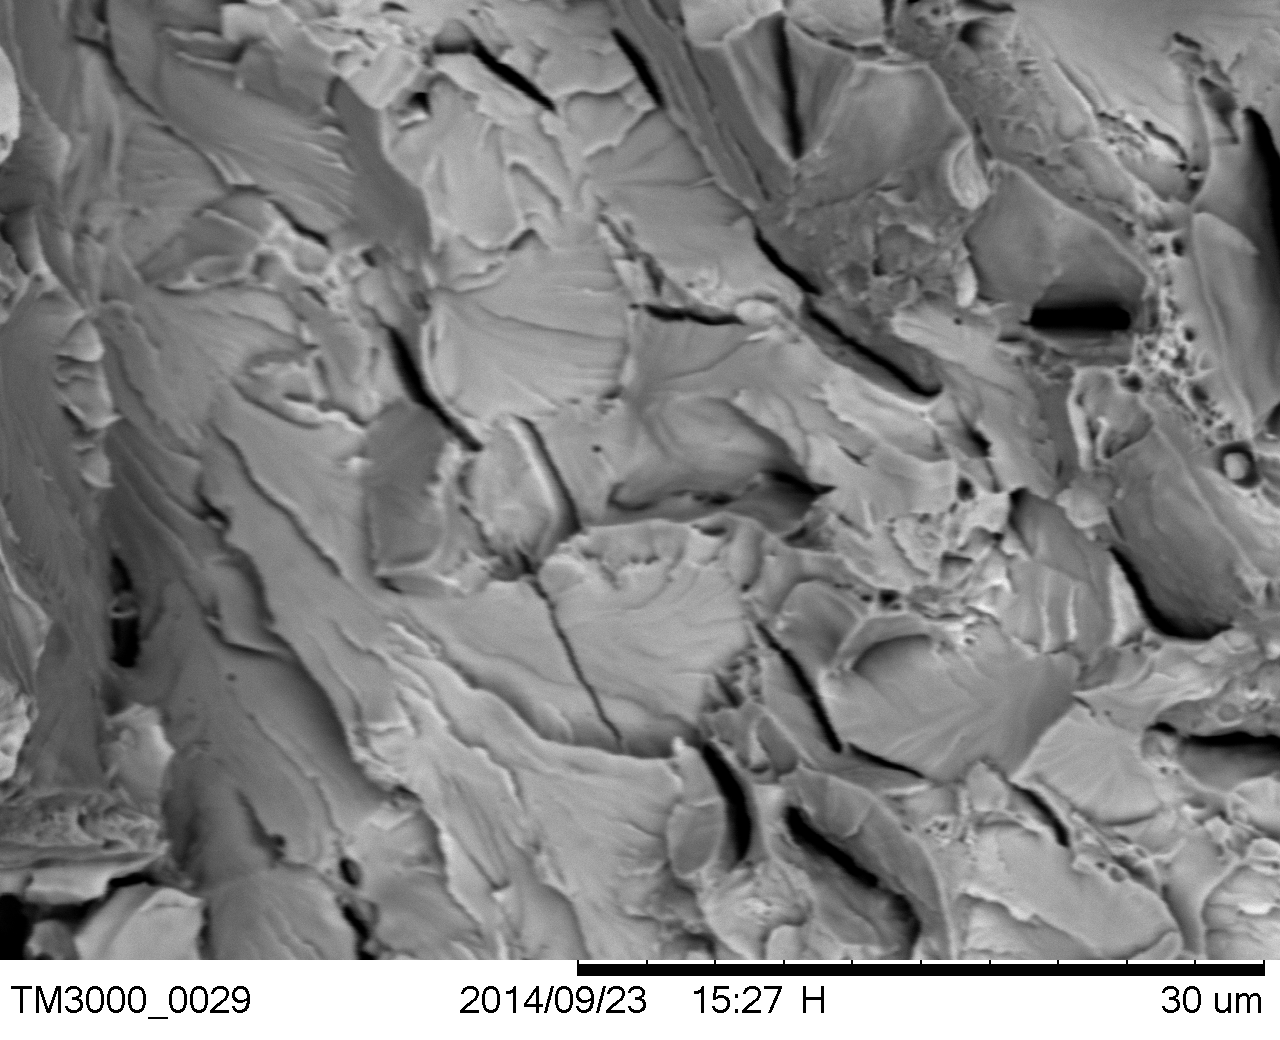
\includegraphics[width=200pt]{graphs/LN2.png}};
\node at (8,0) {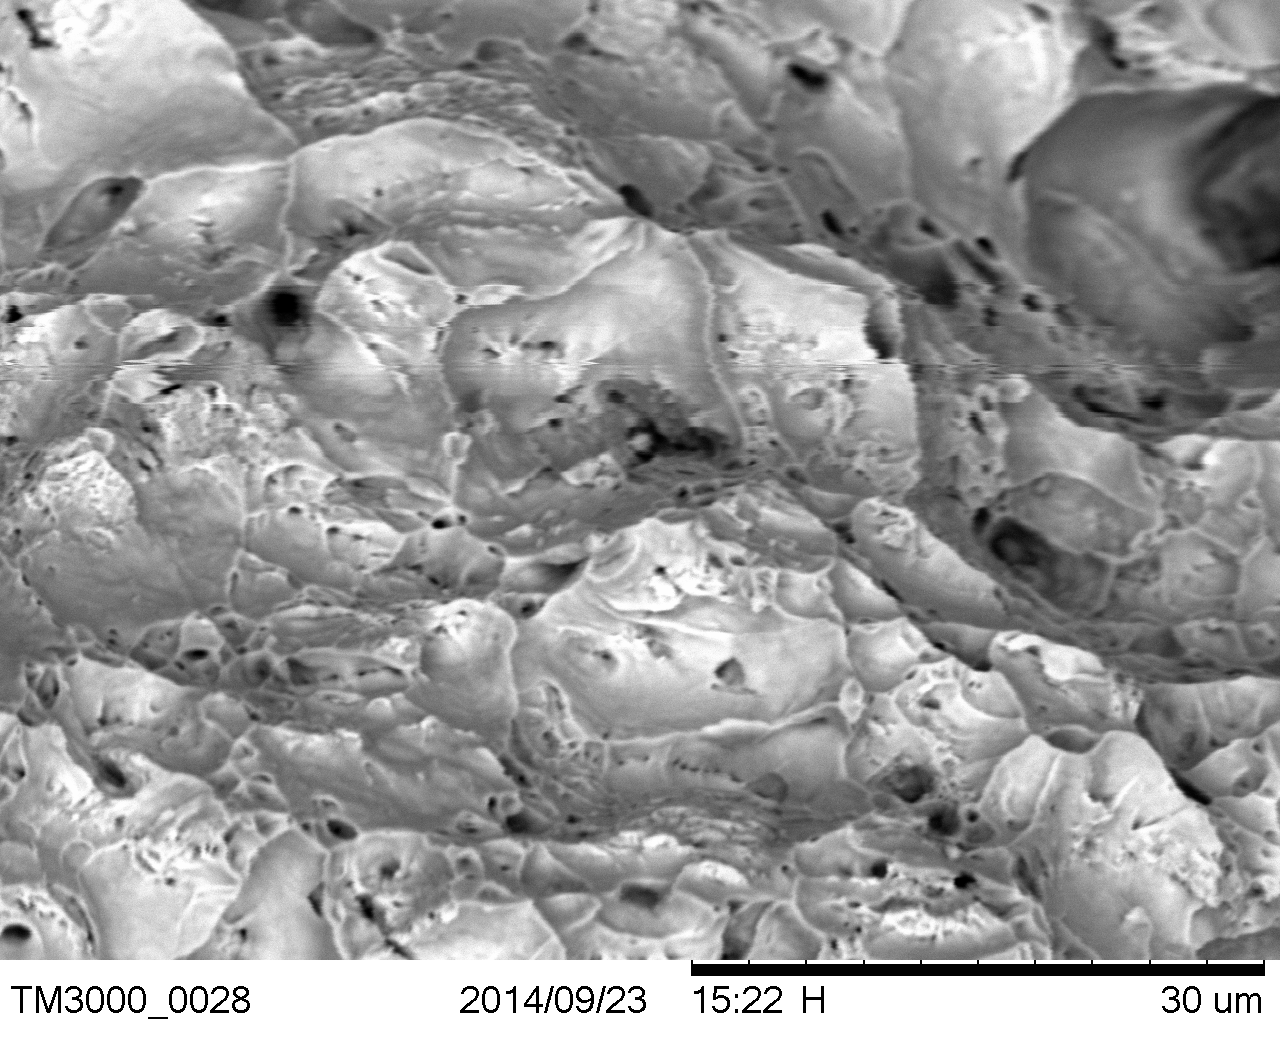
\includegraphics[width=200pt]{graphs/RT.png}};
\node at(0,-3.3) {\textbf{(a)}};
\node at(8,-3.3) {\textbf{(b)}};
\end{tikzpicture}
\caption{\textbf{(a)} SEM picture for Steel-1018. \textbf{(b)} SEM picture for Steel-1018}
\end{figure}

%\begin{figure}[H]
%\centering
%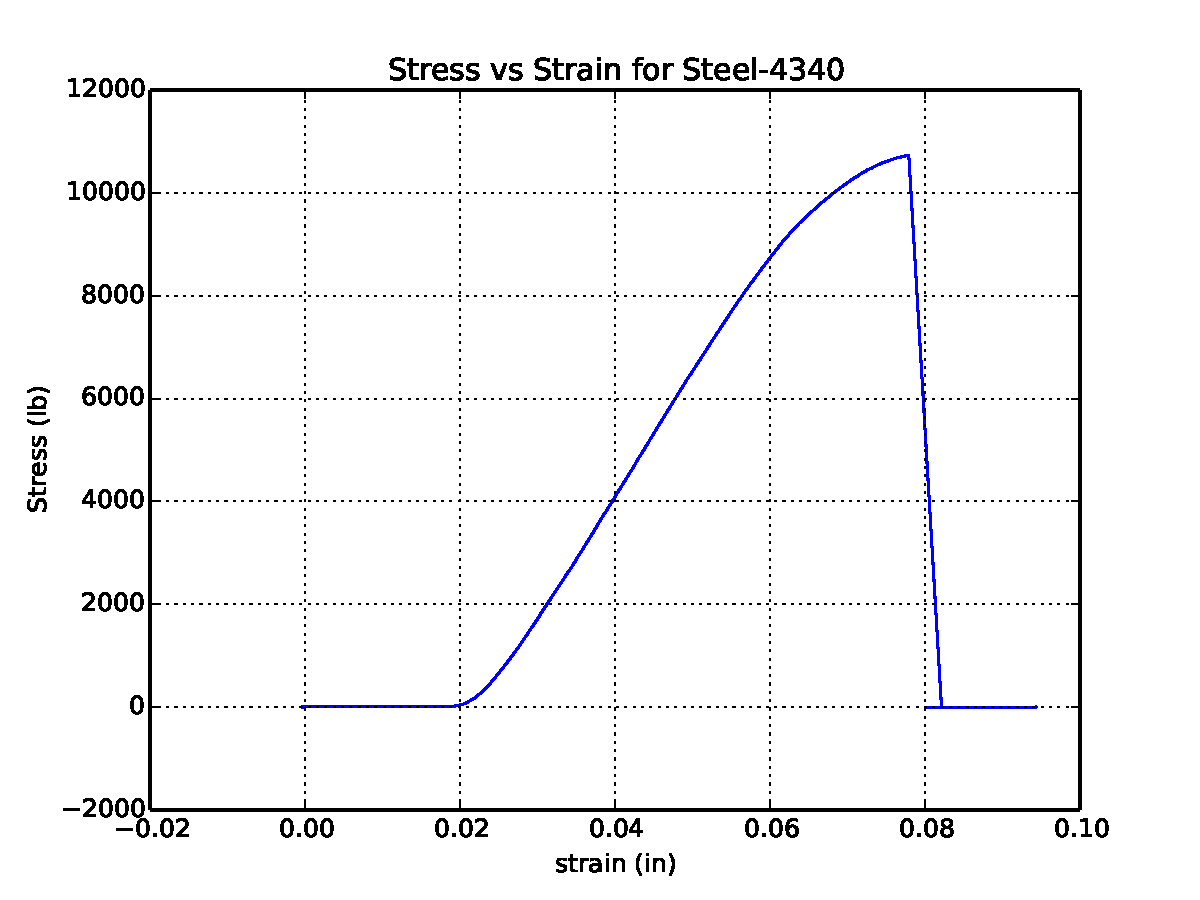
\includegraphics[width=225pt]{graphs/4340.pdf}
%\caption{Charpy test results for Steel-1018}
%\end{figure}

%\begin{figure}[H]
%\centering
%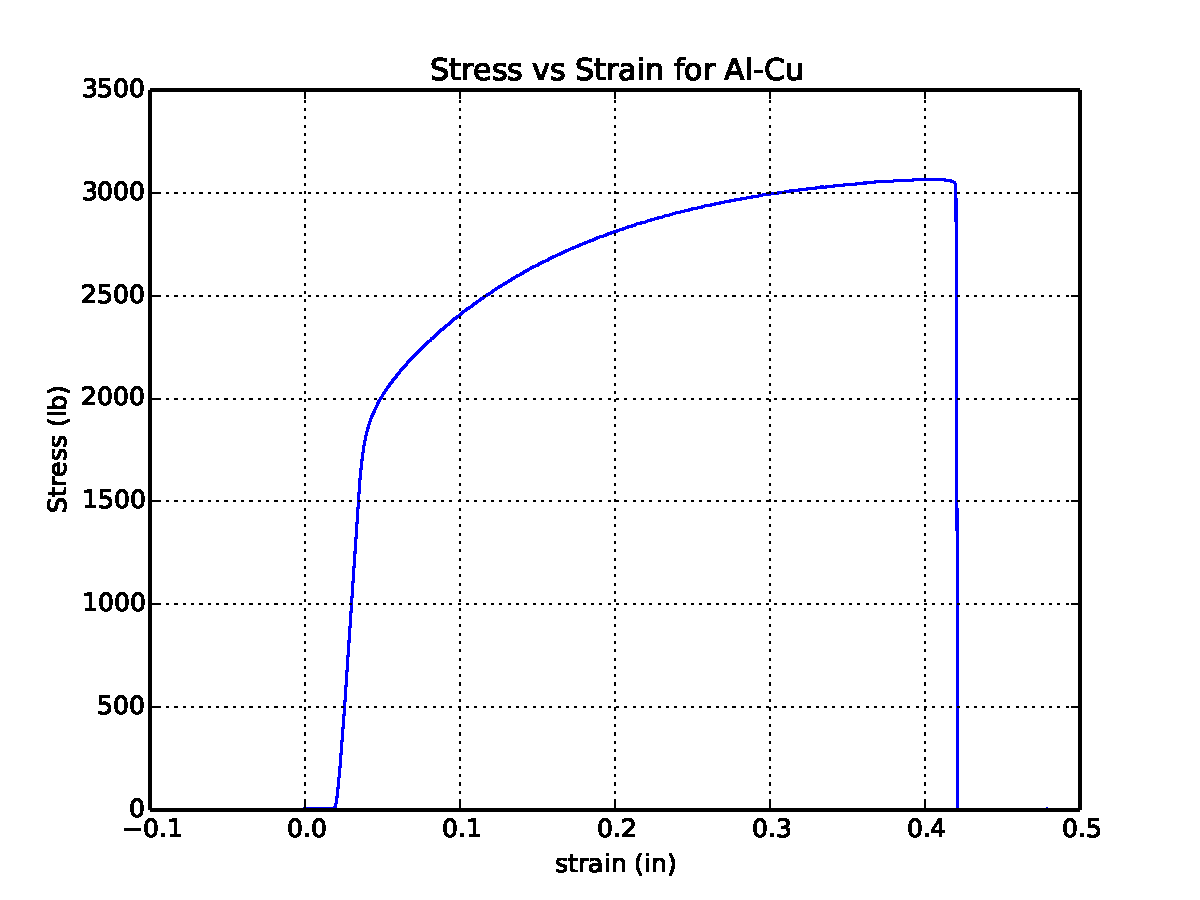
\includegraphics[width=225pt]{graphs/alcu.pdf}
%\caption{Charpy test results for Steel-1018}
%\end{figure}
%----------------------------------------------------------------------------------------
%	SECTION 3
%----------------------------------------------------------------------------------------

\section{Discussion}

\begin{description}[style = nextline]
\item[1) How can you plot an “engineering stress-strain curve” from “applied load” vs “elongation” data. Using your own data, plot engineering stress-strain curves for all three samples and explain. ]
Since we want an engineering stress-strain curve and not just a stress-strain, we need to calculate the initial cross sectional area of the material, $A_0$ and the initial length $l_0$. Next divide these by the 'applied load' and 'elongation' data points in order to get engineering stress-strain data points. Finally plot this new data with your plotting tool of choice. In this case, python.

\begin{figure}[H]
\centering
\begin{tikzpicture}
\node at (0,0) {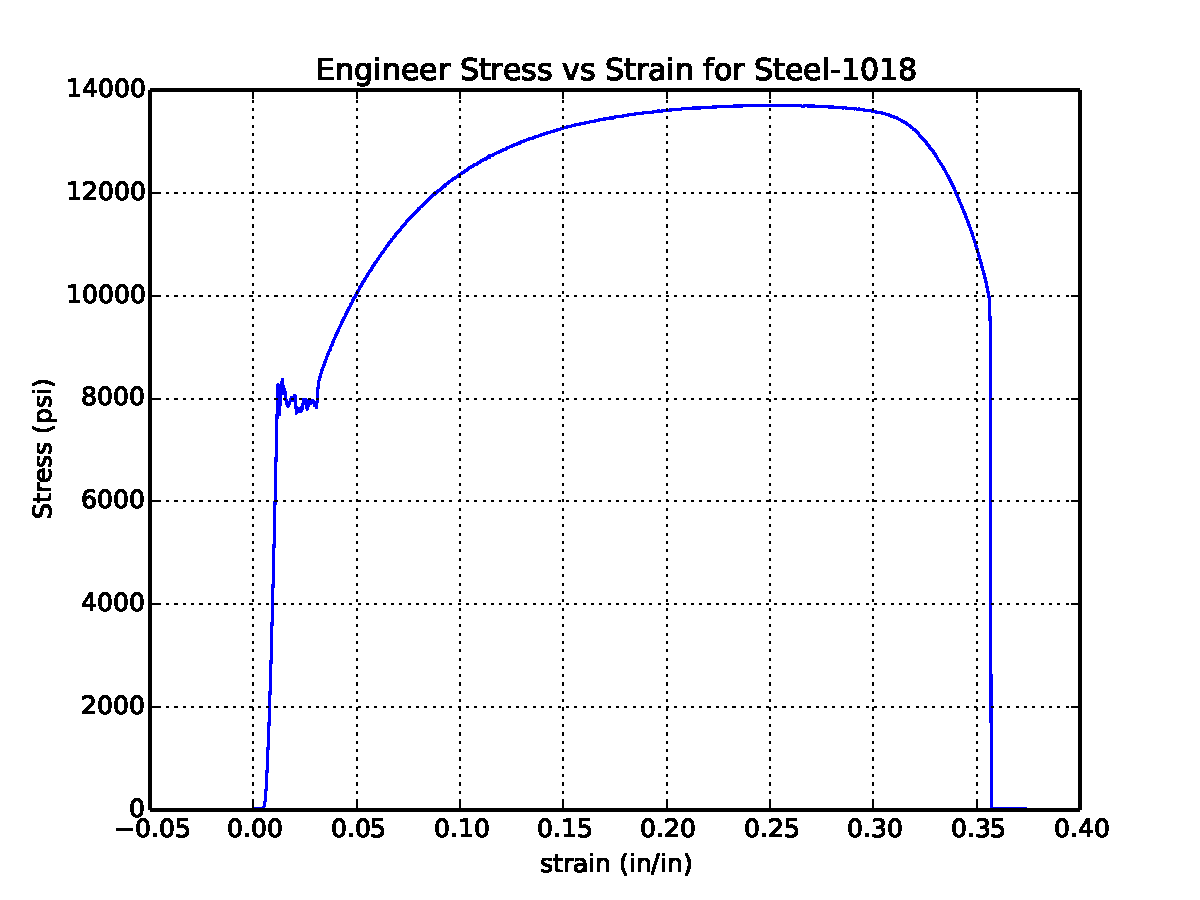
\includegraphics[width=225pt]{graphs/1018e.pdf}};
\node at (8,0) {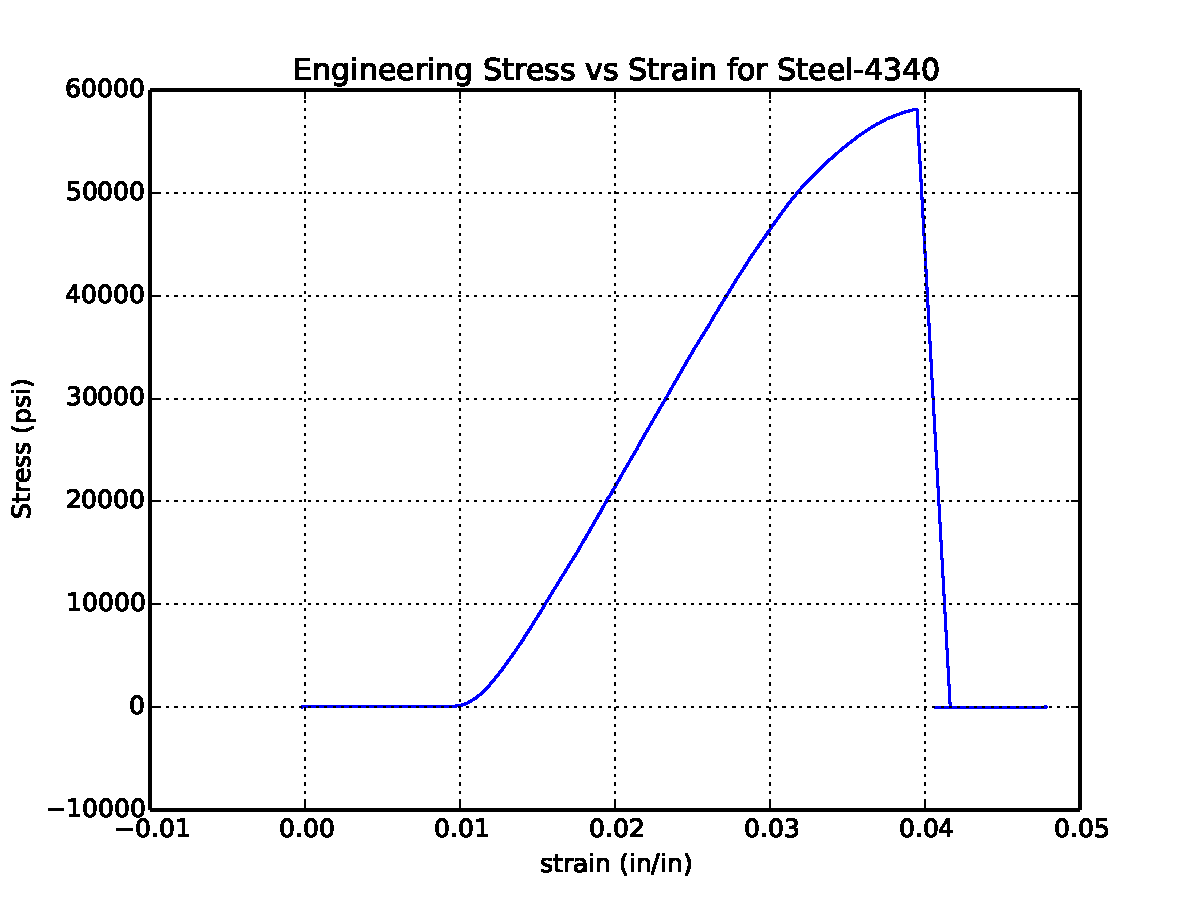
\includegraphics[width=225pt]{graphs/4340e.pdf}};
\node at (4,-6) {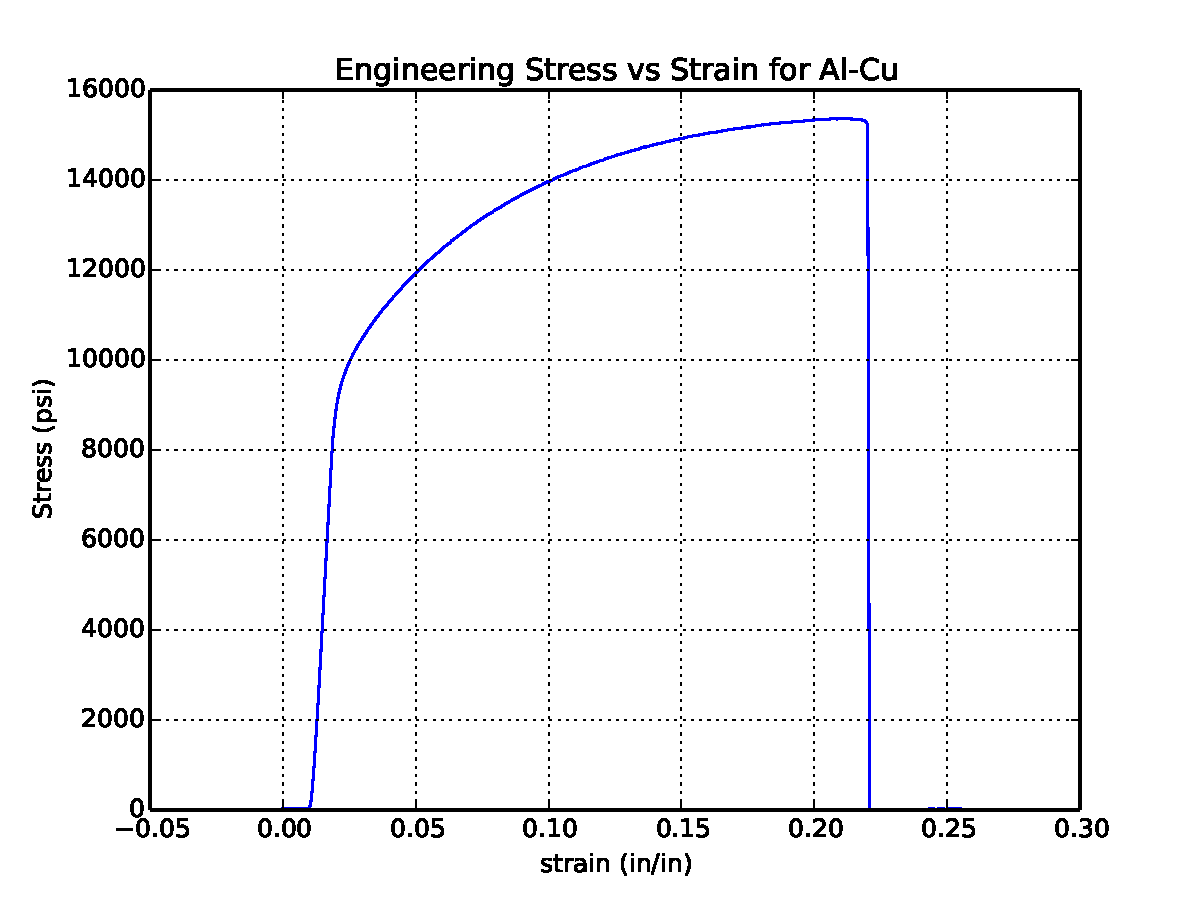
\includegraphics[width=225pt]{graphs/alcue.pdf}};
\node at (0,-3.3) {\textbf{(a)}};
\node at (8,-3.3) {\textbf{(b)}};
\node at (4,-9.3) {\textbf{(b)}};
\end{tikzpicture}
\caption{\textbf{(a)} Engineering Stress-Strain plot results for Steel-1018 using the uniaxial tensile test. \textbf{(b)} Engineering Stress-Strain plot for results Steel-4340 using the uniaxial tensile test. \textbf{(c)} Engineering Stress-Strain plot results for Al-Cu alloy using the uniaxial tensile test.}
\end{figure}

\item[2) From this curve calculate the following for each of the samples: (a) Young's modulus (slope of elastic portion of the curve); (b) yield strength (lower yield strength for steel, 0.2\% offset for aluminum alloy); (c) ultimate tensile strength; (d) fracture stress; (e) percent reduction in area at fracture; (f) total elongation; and (g) toughness (approximated as area under the curve). Explain any anomalies in your results.]
The results all seem to be reasonable. No anomalies that stick out.

\begin{figure}[H]
\centering
\begin{tabular}{c || c | c | c | c | c | c | c}
Material & \specialcell{Young's \\ modulus \\ (psi)} & \specialcell{yield \\ strength \\ (psi)} & \specialcell{ultimate \\ tensile strength \\ (psi)} & \specialcell{fracture \\ stress \\ (psi)} & \specialcell{\% reduction \\ in area at \\ fracture} & \specialcell{total \\ elongation \\ (in/in)} & \specialcell{toughness \\ ($\text{in}^2$)} \\ \hline

Steel-1018 & 1.433629\e{6} & 7.821898\e{3} & 1.370663 \e{4} & 1.12 \e{4} & 88.4 & 0.315 & 4.311251 \e{3} \\ \hline
Steel-4340 & 2.624936\e{6} & 52.25604 \e{3} & 5.812479 \e{4} & 5.84 \e{4} & 99.6 & 0.0177 & 1.006291 \e{3} \\ \hline
Al-Cu & 1.057670 \e{6} & 9.127436\e{3} & 1.536832 \e{4} & 1.67 \e{4} & 91.3 & 0.192 & 2.819101 \e{3} \\ \hline
\end{tabular}
\caption{Table shows the key mechanic properties of a tensile test for two types of steel and a Al-Cu alloy. Some of the results has 7 sig figs because the uniaxial test data provided 7 sig figs of accuracy. The measurements of area and length were done in 3 sig figs because this was measured with a XXX.}
\end{figure}

\item[3) During the tensile test the volume of the material remains constant, which can be expressed mathematically as, $l_0A_0 = l_iA_i = \text{constant}$. Using this relation and the definitions of engineering stress, engineering strain, true stress, and true strain, derive the following relationship between true stress and engineering stress, $\sigma_{\text{true}} = \sigma_e(1 + \epsilon_e)$, and the relationship between true strain and engineering strain, $te\epsilon_{\text{true}} = \sigma_e(1 + \epsilon_e)$.]

\begin{equation}
\sigma_{\text{true}} = \frac{P}{A_i} = \frac{Pl_i}{A_0l_0} = \sigma_e\frac{l_i}{l_0} = \sigma_e\frac{l_0 + l_0\epsilon_e}{l_0} = \sigma_e(1 + \epsilon_e)
\end{equation}
\begin{equation}
\epsilon_{\text{true}} = \ln{\frac{l_i}{l_0}} = \ln{\frac{l_0 + l_0 \epsilon_e}{l_0}} = \ln{(1 + \epsilon_e)}
\end{equation}

\item[4) Convert your engineering stress-strain curves to true stress-strain curves.]
See figure 7 below.

\begin{figure}[H]
\centering
\begin{tikzpicture}
\node at (0,0) {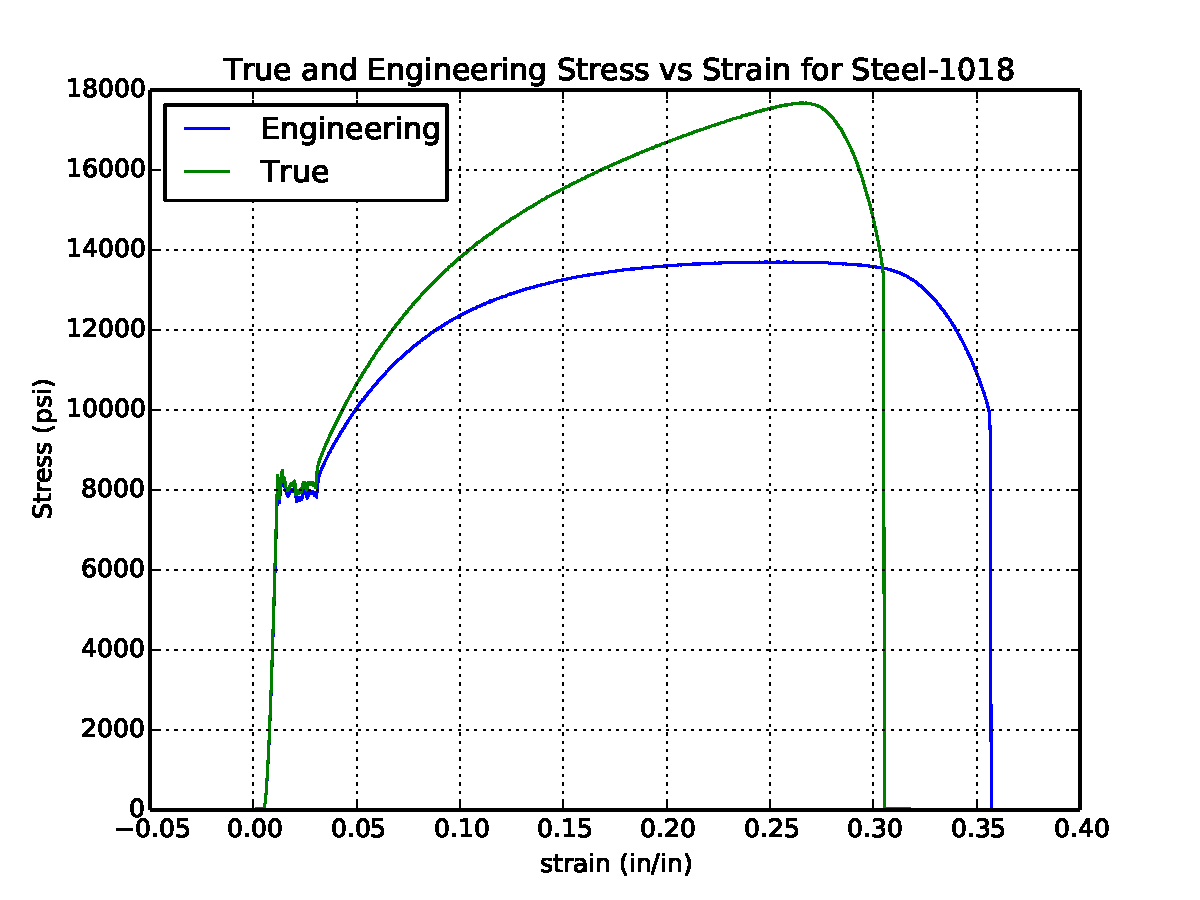
\includegraphics[width=225pt]{graphs/1018et.pdf}};
\node at (8,0) {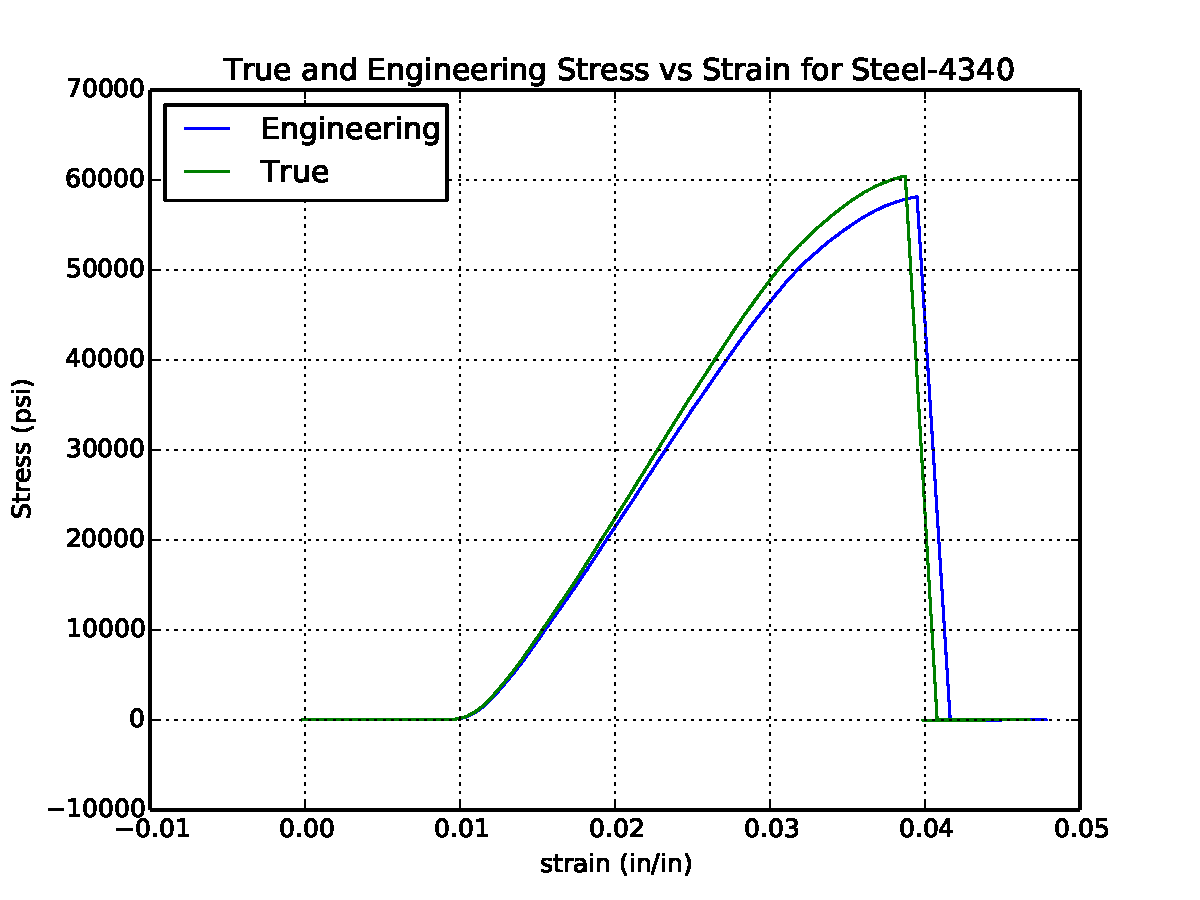
\includegraphics[width=225pt]{graphs/4340et.pdf}};
\node at (4,-6) {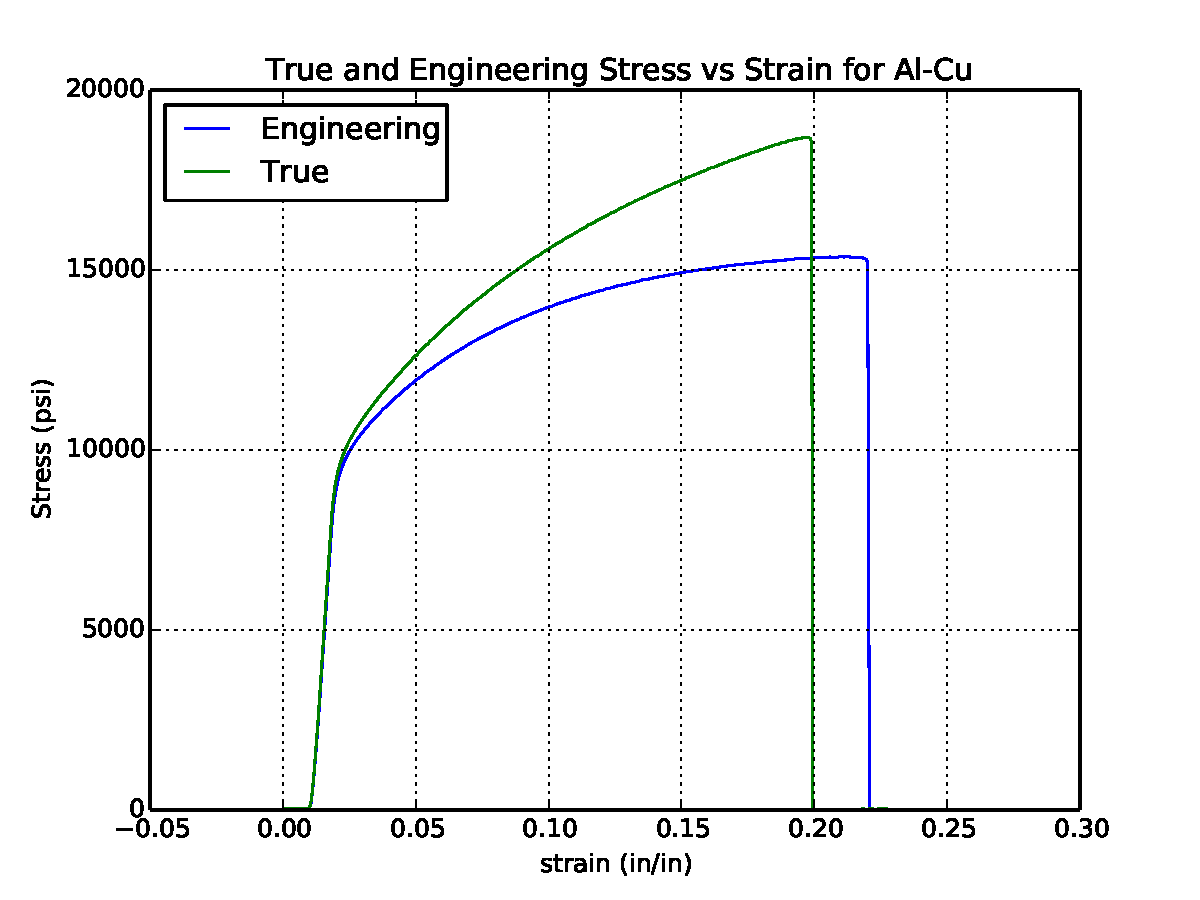
\includegraphics[width=225pt]{graphs/alcuet.pdf}};
\node at (0,-3.3) {\textbf{(a)}};
\node at (8,-3.3) {\textbf{(b)}};
\node at (4,-9.3) {\textbf{(b)}};
\end{tikzpicture}
\caption{Both true and engineering plots were overlayed in order to better see the comparation between the two. \textbf{(a)} True and Engineering Stress-Strain plot results for Steel-1018 using the uniaxial tensile test. \textbf{(b)} True and Engineering Stress-Strain plot for results Steel-4340 using the uniaxial tensile test. \textbf{(c)} Engineering Stress-Strain plot results for Al-Cu alloy using the uniaxial tensile test.}
\end{figure}

\item[5) Where (physical location) on each sample did you observe “necking” to occur? Is this where you expected to see it? Explain.]
I expected necking as well as fracture to occur where the initial rockwell tests were done, near the ends of the materials. For the Al-Cu alloy necking and fracture did occur at the end of the material, but for the two steel samples, necking and fracture occuring more towards the center than the ends. There was much more necking (clearly visible in Figure 8) on the Steel-1018 sample than the Steel-4340 sample; this is also verified by looking at the plots in Figure 7.

\begin{figure}[H]
\centering
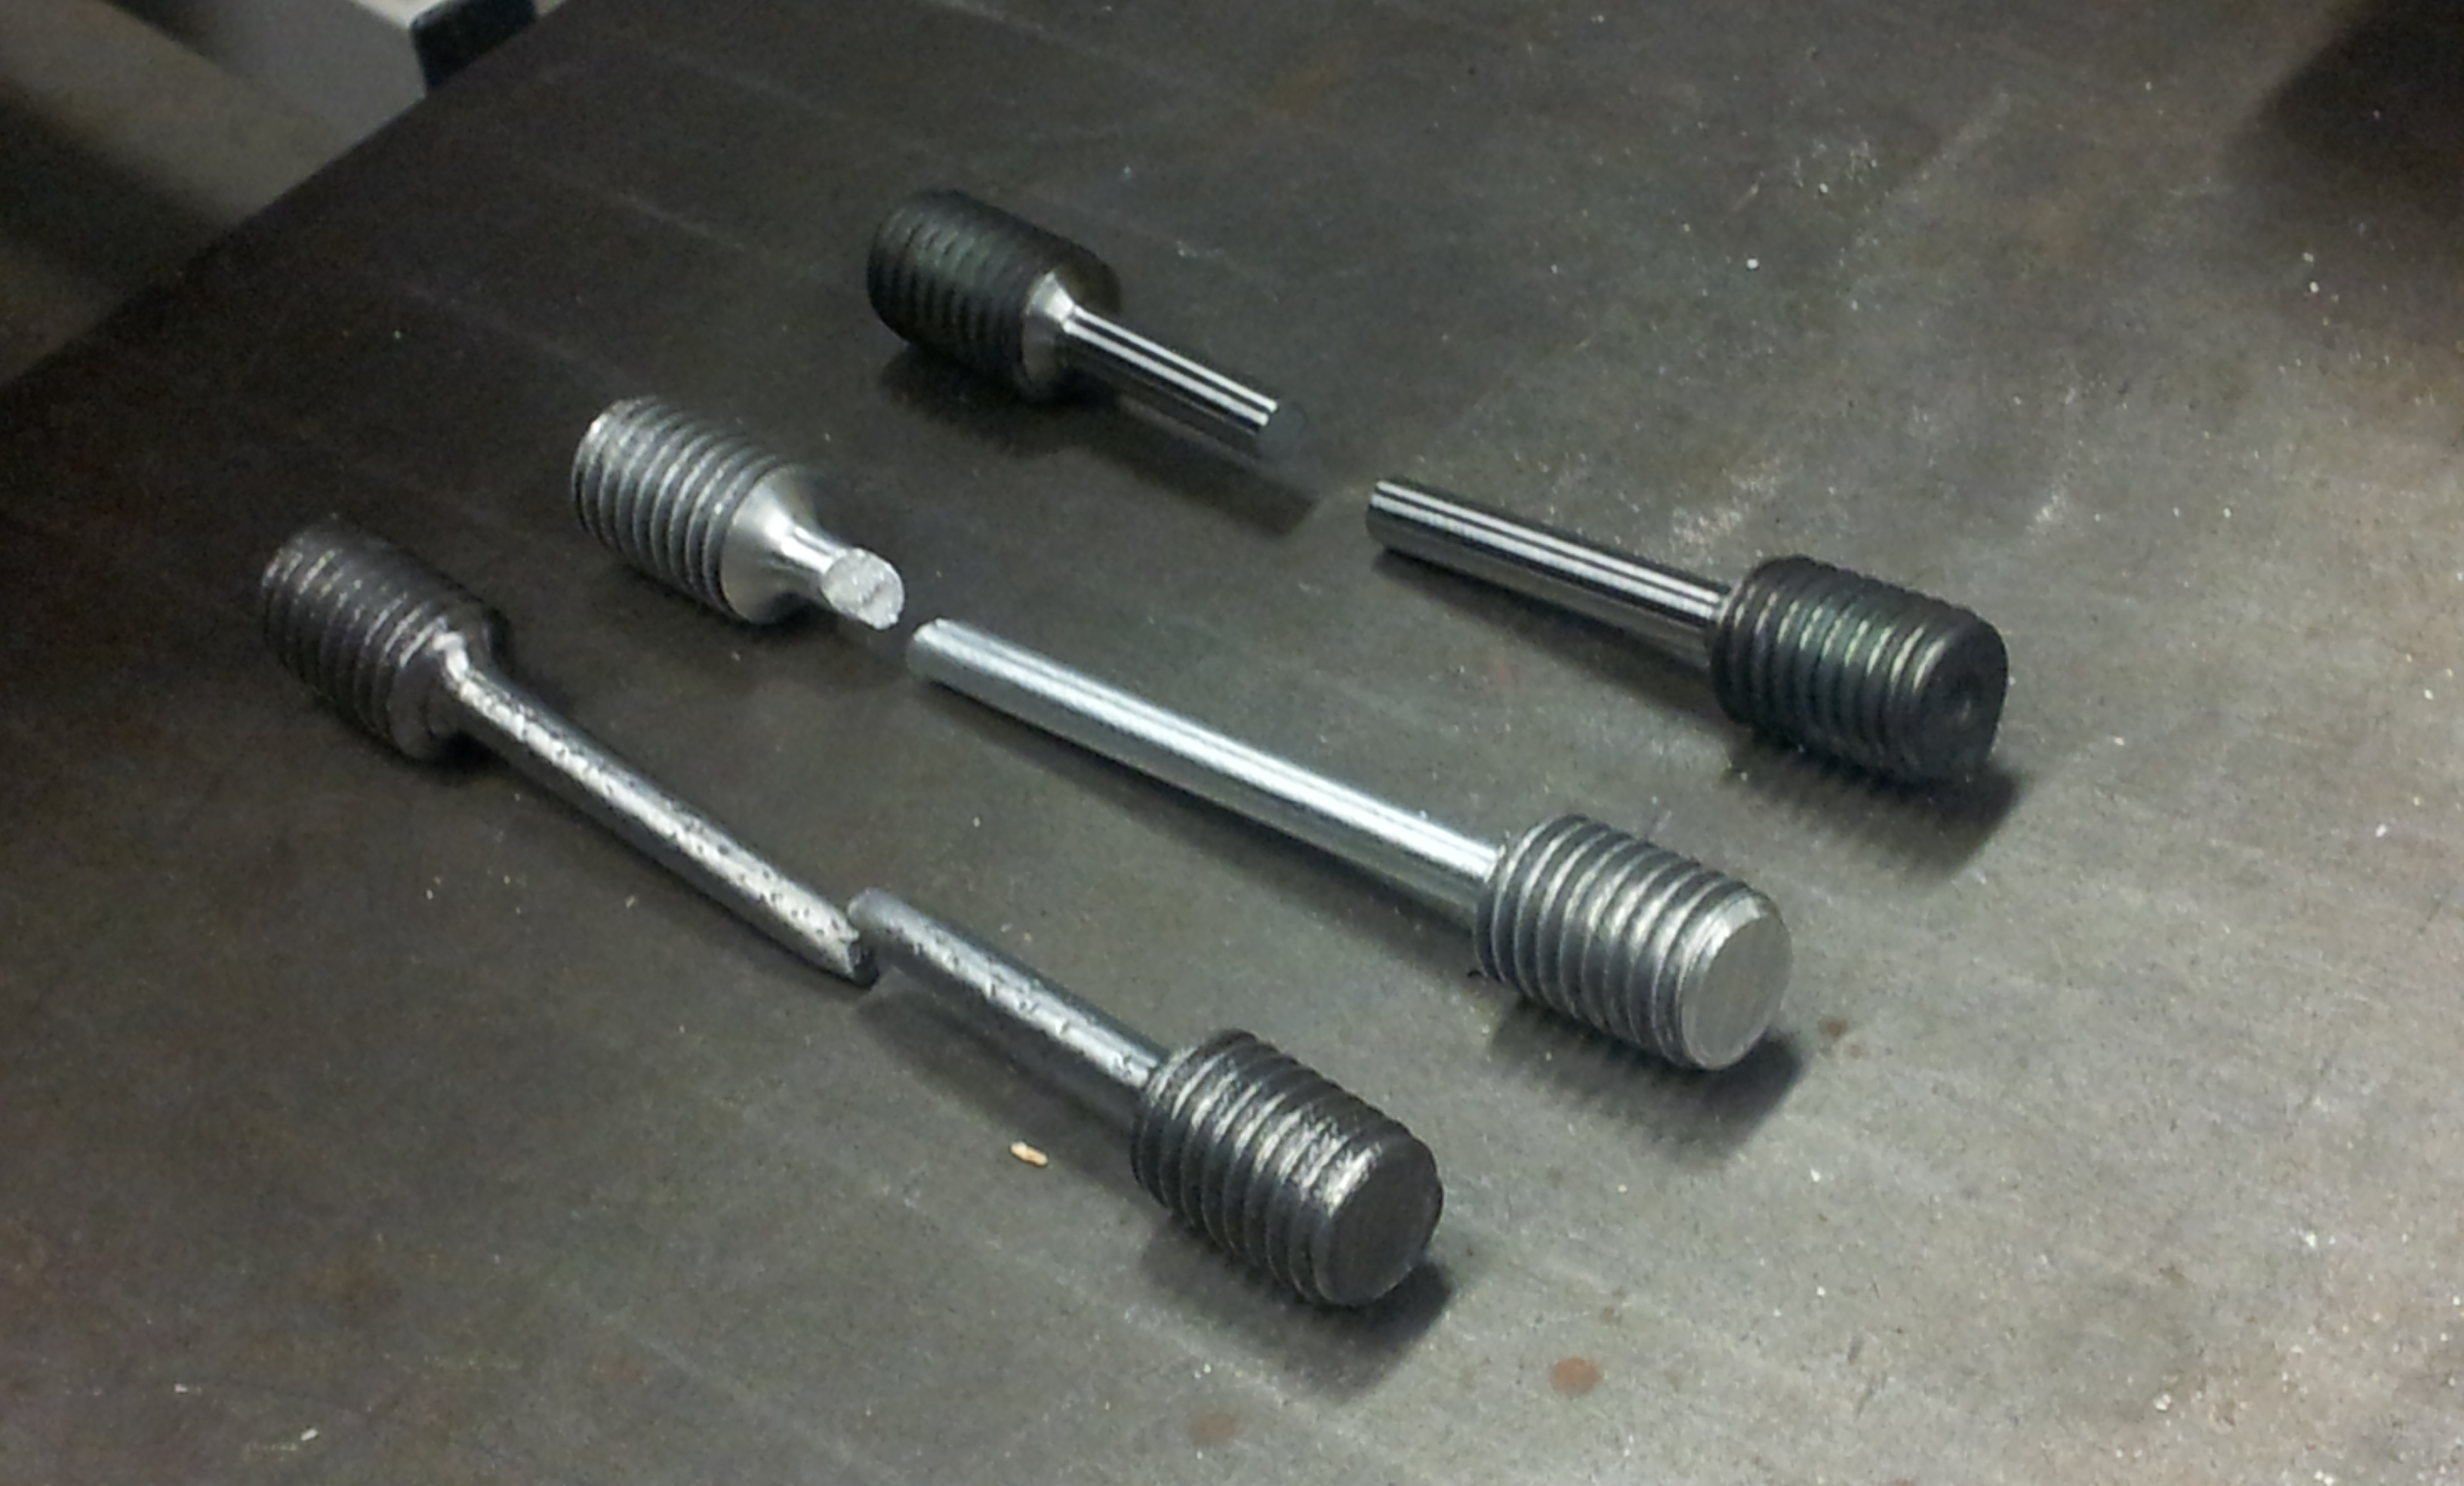
\includegraphics[width=200pt]{graphs/samplepic.jpg}
\caption{Samples used for the uniaxial tensile test. From left to right: steel-1018, Al-Cu, steel-4340. Note the necking in steel-1018 is clearly visible in this picture.}
\end{figure}

\item[6) Compare and contrast the scanning electron “fractographs” recorded during your lab experiments. What are the distinctive features of the fracture surface? How do these features differ from sample to sample? Do these observations make physical sense with respect to their observed strength and toughness? Explain.]
\end{description}
%----------------------------------------------------------------------------------------
%	SECTION 4
%----------------------------------------------------------------------------------------

\section{Conclusions}
As a result of this investigation, the following conclusions can be drawn.
\begin{enumerate}
\item The rockwell and brinell tests do adequetly provide a way to measure a materials hardness.
\item Alloys tend to have a higher hardness number than metals meaning that they are much stronger materials.
\item Holes in materials significantly affect that materials tensile strength.
\item Depending on the radius of curviture, stress on holes can vary significantly.
\end{enumerate}

%----------------------------------------------------------------------------------------
%	SECTION 5
%----------------------------------------------------------------------------------------

\section{References}
\begin{enumerate}
\item James F. Shackelford, Introduction to Materials Science for Engineers, Seventh Edition, Pearson Higher 
Education, Inc., Upper Saddle River, New Jersey (2009).
\end{enumerate}

%----------------------------------------------------------------------------------------
%	SECTION 6
%----------------------------------------------------------------------------------------

% Nothing right now

%----------------------------------------------------------------------------------------
%	BIBLIOGRAPHY
%----------------------------------------------------------------------------------------

\bibliographystyle{apalike}

\bibliography{sample}

%----------------------------------------------------------------------------------------


\end{document}

